\chapter{Analytics Tools used in this research}
\label{appendix-analytics-tools}

This chapter complements the `On Mobile Analytics` chapter. That chapter covers the key elements and concepts, this one describes the analytics tools we used during my research.

\begin{itemize}
    \item Android Vitals (integrated into Google Play Console)
    \item AppPulse Mobile (when owned by HP)
    \item Azetone heat mapping together with some collaboration with Appsee
    \item count.ly
    \item Crashlytics (when owned by Google and branded as Fabric, and briefly after it was migrated to Firebase)
    \item Flight Recorder (now defunct)
    \item Iteratively
    \item Microsoft App Center
    \item Google Firebase Analytics
    \item Google Play Console (2018-2020 and 2020-2021 editions)
\end{itemize}

\section{AppPulse Mobile}

Open API \href{https://github.com/MicroFocus/apmobile-openapiclient/blob/master/doc/AppPulse_Mobile_Open_API_Guide.pdf}{Open API Guide} and a  \href{https://github.com/MicroFocus/apmobile-openapiclient}{sample client for AppPulse Mobile's Open API}

``Open API – Resource Usage: Extract battery usage and cellular usage data to create custom reports integrated with external systems and dashboards. New APIs help you mine resource usage metrics from your user’s devices and operating systems." from ``What's New in AppPulse Summer '16 Release"

\begin{itemize}
    \item ``...tested an hybrid application, this requires to turn a special flag in the instrumentation process, I assume it wasn’t turned on and that is the reason for not capturing some of the things." However: the \texttt{-hybrid} instrumentation flag which doesn't actually seem to exist in 1.96, perhaps it's only in a pre-release version
    \item ``AppPulse mobile requires internet access from the mobile device. We monitor the user actions, crashes etc. and report the statistics back to HP SaaS servers – sending the data is done over the internet."
    \item HP have made improvements to AppPulse Mobile as a result of working with me, so their library now captures more of the user actions (Sept 2015).
\end{itemize}

Findings: 
\begin{enumerate}
    \item How well does the client library cope in terms of storing and subsequently forwarding events, messages, whatever, in the following circumstances?
    \begin{enumerate}
        \item Use of a proxy server?
        \item When connected to a Wi-Fi that doesn't have internet access e.g. a local internal hotspot?
        \item When the network is unavailable e.g. when the device is in 'flight mode' without Wi-Fi or mobile network access?
    \end{enumerate}
    \item I saw an example where my app crashed on an Android 2.3 device (and old Google Nexus One) where AppPulse Mobile didn't record the crash.
    \item The FunDex score varied more than I expected, and sometimes changed as I navigated around the various sections of the UI. A pattern seemed to start to emerge but I didn't test it sufficiently to describe it accurately.
    \item Some UI events, and other events, don't seem to be captured by AppPulse Mobile. Examples include:
    \begin{enumerate}
        \item Read aloud text on the screen (triggered from a menu option)
        \item Navigation in a WebView
        \item Changing ease of access settings and other UI preferences
    \end{enumerate}
\end{enumerate}

I'd also appreciate knowing more about the data transmission aspect, such as message sizes, frequency of sending, whether it aggregates several events into a single transmission, etc.

BTW: I wonder how much it's been used with apps that support multiple UI languages (Kiwix for Android supports 100+). The screen labels are sometimes derived from the display language so they seem to be treated as separate elements in the user flows.]

Results:
\begin{itemize}
    \item The development team of the Analytics tool observed: ``I instrumented the apk, in general the instrumentation works. I do see some gaps, some missing actions, it’s because the application loads the content from the local file system - it seems that sometimes we don’t inject the instrumentation fast enough. I investigating it now and will let you know about the progress. [The] -hybrid flag is used in the java code internally, the shell script just passes the parameters." % Email source: https://mail.google.com/mail/u/0/#search/apppulse+mobile/FMfcgxmMlGKpJrtjFNcbGDcwpvBHHBjv
    \item [I discovered] AppPulse Mobile did not deliver events that occurred when the device had no internet connection. I proposed improvements to the AppPulse Mobile SDK so that it would store timestamped events locally and transmit them when the network connection was available. The improvements included considerations on the server-side processing of delayed events. %Original notes follow, the email source is: https://mail.google.com/mail/u/0/#search/apppulse+mobile/FMfcgxmNwpbfZkVPJpqFPrKMZjTjwxGW
    \item A bug in an analytics SDK didn't release memory for objects while scrolling a very long image list ( cart list) which caused the app to crash in production. An unanswered question was whether the built APK file was checked after the crashes occurred to determine whether optimisation practices such as zipalign were run correctly on it \url{https://developer.android.com/studio/command-line/zipalign.html} which reduces the memory footprint at runtime. Sources private correspondence with the SDK provider % https://mail.google.com/mail/u/0/#search/apppulse+mobile/FMfcgxmQHnbPSVLJShFHXvrxlccmzrJD
\end{itemize}

\begin{comment}
I've asked earlier to see if you could get AppPulse Mobile to be able to collect data (the analytics events) when there's no suitable network available, and where the data is safely recorded locally on the mobile device until such time as a viable network connection is available, then the data would be transmitted to the receiving AppPulse Mobile servers.

There are some design implications. Here are the main ones I consider:
Timestamping of event records. Perhaps the event records are already timestamped. If not, they, and their timestamps need to be transmitted, if we want to accurately process them.
Reporting of the data. As some data may arrive hours or even days after data that's been sent synchronously (from devices that had a working network connection), then reports may need to be recalculated and possibly retransmitted (and available as an update via the Open API's). There may need to be cutoffs in the system, possibly in the acceptance of 'old' data, possibly in the automated reports, possibly elsewhere.
How much data would be stored for how long on the local devices? FYI IIRC one of the similar genre of mobile analytics stores 5 discrete crashes while offline. Any more cause some data to be discarded. I don't know the details. It would be possible to calculate summary statistics and transmit those in cases where the AppPulse Mobile library has exceeded it's design/implementation/runtime storage limit(s). I'd hope the data could be stored for long periods and in relatively large volumes in terms of records. There are various techniques available to compress the data that's transmitted.
Having offline collection can help capture usage data and usage patterns that occur when the network is not available. In some cases the patterns may only happen when there's no viable network. For instance, apps may offer specific functionality when working in 'offline mode'.

Various competitors include support for offline data collection. My expectation is that as more people use AppPulse Mobile some will discover the lack of offline data collection and cause them to adversely consider the product as a result.
\end{comment}

\section{Heatmapping: Azetone and Appsee}

hotjar.com article on 8 tests using heatmaps.

\subsection{Azetone (in 2015)}
\begin{itemize}
    \item ``by default our SDKs are reporting back to the servers with a delay which can be up to 15 hours (to minimize bandwidth and resource consumption)"
    \item  \texttt{IntentReceiver com.immersion.android.haptics.HapticFeedbackManager\$HapticFeedbackBroadcastReceiver@41d4fe50} integrated into their Android SDK
    \item Record in admin mode ``make sure you use connect to your App in Admin mode to gather the different screens you want Heatmaps on…"
    \item Configuration options: optional call to increase the level of logging, explicit call to set the dispatch period to 240 seconds,
    \item Flaws in the reports: A system that's never been used should indicate it's never been used and is 'at-rest', whereas I've currently used (got) 20 users and even improvements on last month. application's name still appears as abcdef in the dashboard
\end{itemize}
Sources include email correspondence and my notes at the time.

\href{https://www.azetone.com/mobile-ux-analytics/}{Understand, Optimize and Personalize your UX - UX Analytics for iOS and Android}

\begin{figure}
    \centering
    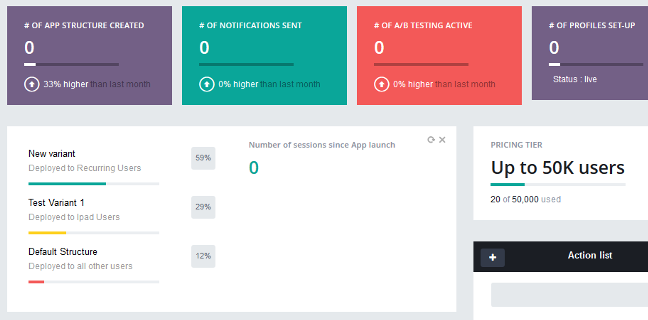
\includegraphics[width=16cm]{images/azetone/azetone_dashboard_flaws_for_kiwix_2015.png}
    \caption{Azetone flaws in the dashboard}
    \label{fig:azetone_dashboard_flaws_for_kiwix_2015}
\end{figure}



\subsection{AppSee (in 2015)}
Individual recordings, aggregate heatmaps: Slide 4: ``Visualize both single user data (user replay) and aggregated user behaviour (touch heatmaps)" This point is insightful, and explains how both individual information and aggregate information are relevant and useful.

Slide 5: I like the comparison between "Gives the Why" and "Gives the What". However I think the quote favours themselves (as one might expect) and underplays how other mobile analytics can help. Also, from a privacy perspective, there's a general dislike and disquiet about such intrusive monitoring (visual monitoring, recording interactions, etc.) I sent you the spreadsheet with the results from my questionnaire on 17th, so app developers need to carefully consider whether visual analytics is worth the extra bandwidth usage and intrusion into users' privacy. 



AppSee far more polished than Azetone.
\href{https://youtu.be/GQ2DoINkba4?t=554}{Appsee-Optimizely Webinar: How to Perform the Ultimate A B Test with UX Analytics}

\url{https://medium.com/@Appseecom}

\url{https://www.slideshare.net/SafeDK/how-to-work-compliantly-with-3rd-parties}

SafeDK published a short video on YouTube that explains how libraries are not your code yet you are responsible as an app developer for the libraries you include. Their SDK at the time (2015) enabled developers to have fine-grained near real-time control over aspects of the libraries embedded in their app and also provided analytics on those libraries.

More info: 
http://blog.safedk.com/technology/what-you-should-know-about-your-sdks-and-your-app-start-time/
http://blog.safedk.com/sdk-economy/5-steps-in-choosing-the-right-3rd-party-tools-sdks-for-your-mobile-app/
and http://blog.safedk.com/sdk-economy/do-you-know-what-your-sdks-did-last-summer/



\section{Flight Recorder}
Screen Recording: 
Watch, understand and improve
\begin{itemize}
    \item \textbf{REC} We record screen captures of sessions that show you each and every action your users take drilldown by events and watch the videos that matter.
    \item \textbf{Touches \& Swipes} Recorded and summarized as heat maps. See the most touched areas screen by screen.
    \item \textbf{User Based Sessions} A user centric vision \& action capability to the sessions. You just need to call FlightRecorder SDK's User ID method, that's all.
\end{itemize}
Source: \url{https://web.archive.org/web/20150717030554/http://www.flightrecorder.io/feature/screen-recording}

About Unlimited Crash Reports: 
Every plan has session limits, if you exceed your limits, FlightRecorder runs locally ( by default this option is enabled, you can disable it remotely also ), if a crash occurs, SDK sends all the data for that session. It deletes the recordings and other tracked datas for non-crashed sessions from local.~\url{https://web.archive.org/web/20150717030349/http://www.flightrecorder.io/feature/crash-reporting}

Combined API/HTTP Logs and Exceptions with recordings of app activities. \url{https://web.archive.org/web/20150901043518/https://www.flightrecorder.io/feature/http-requests-and-response-logging}. Touch Heatmaps
Visualize the clicks and swipes of your users and uncover usage patterns. Recorded and summarized as heat maps. See the most touched areas screen by screen.~\url{https://web.archive.org/web/20150823000332/http://flightrecorder.io/feature/touch-heat-maps}

\href{https://web.archive.org/web/20151104224311/http://help.flightrecorder.co/quick-start/}{Flight Recorder: Quick Start Guides for iOS and Android}.

\section{Google Play Console incorporating Android Vitals}\label{google_play_console_section}

\subsection{Key Components of Google Play Console}
\subsubsection{Google Play Console UI}

TODO Describe each screen and the contents. Provide a table of the URL mapping and summary of their contents.

Name each graph and provide a screenshot so they can be discussed.

\begin{figure}[htbp!]
    \centering
    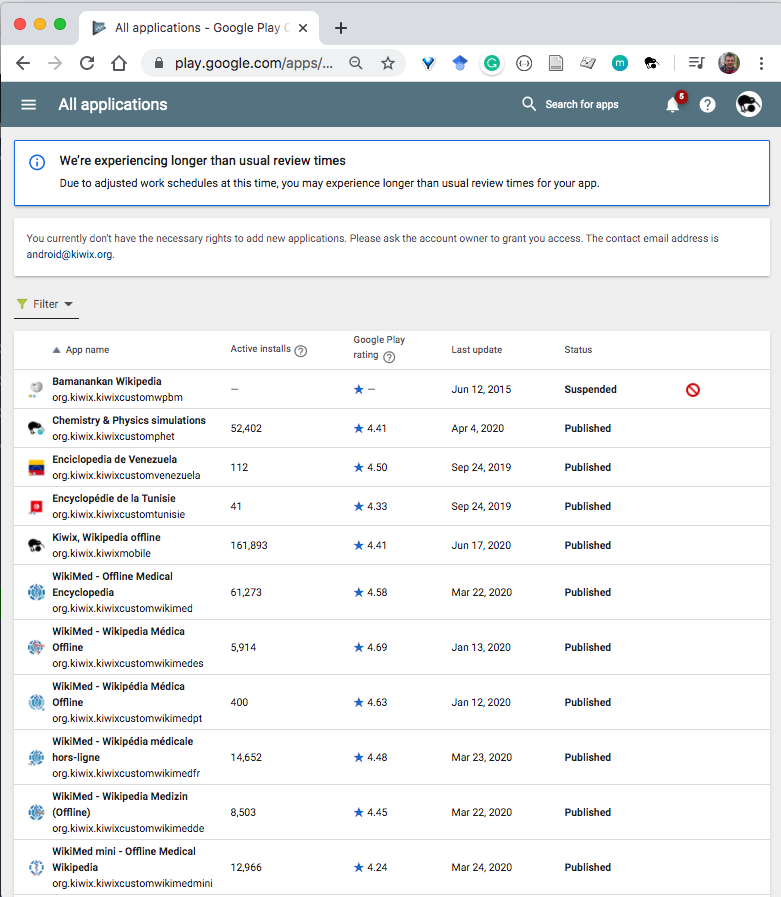
\includegraphics[width=15cm]{images/android-vitals-screenshots/AppListPlace-kiwix-2020-Jun-17.png}
    \caption{Google Play Console: AppListPlace for Kiwix project}
    \label{fig:gpc-applistplace-kiwix}
\end{figure}

\subsubsection{Release Management}
Mobile apps are released in the app store and there are defining events representing the start and end of each release. Releases take time to complete. During the release period the developers have some control on the rollout within the app store (they may also have controls within the app and/or in their related systems and services). Google Play Console provides them with the controls in the app store, it also provides three bands of reports, these are:

\begin{itemize}
    \item Release stability (which leads to Android Vitals)
    \item Ratings and reviews
    \item Installs and uninstalls
\end{itemize}

\begin{figure}
    \centering
    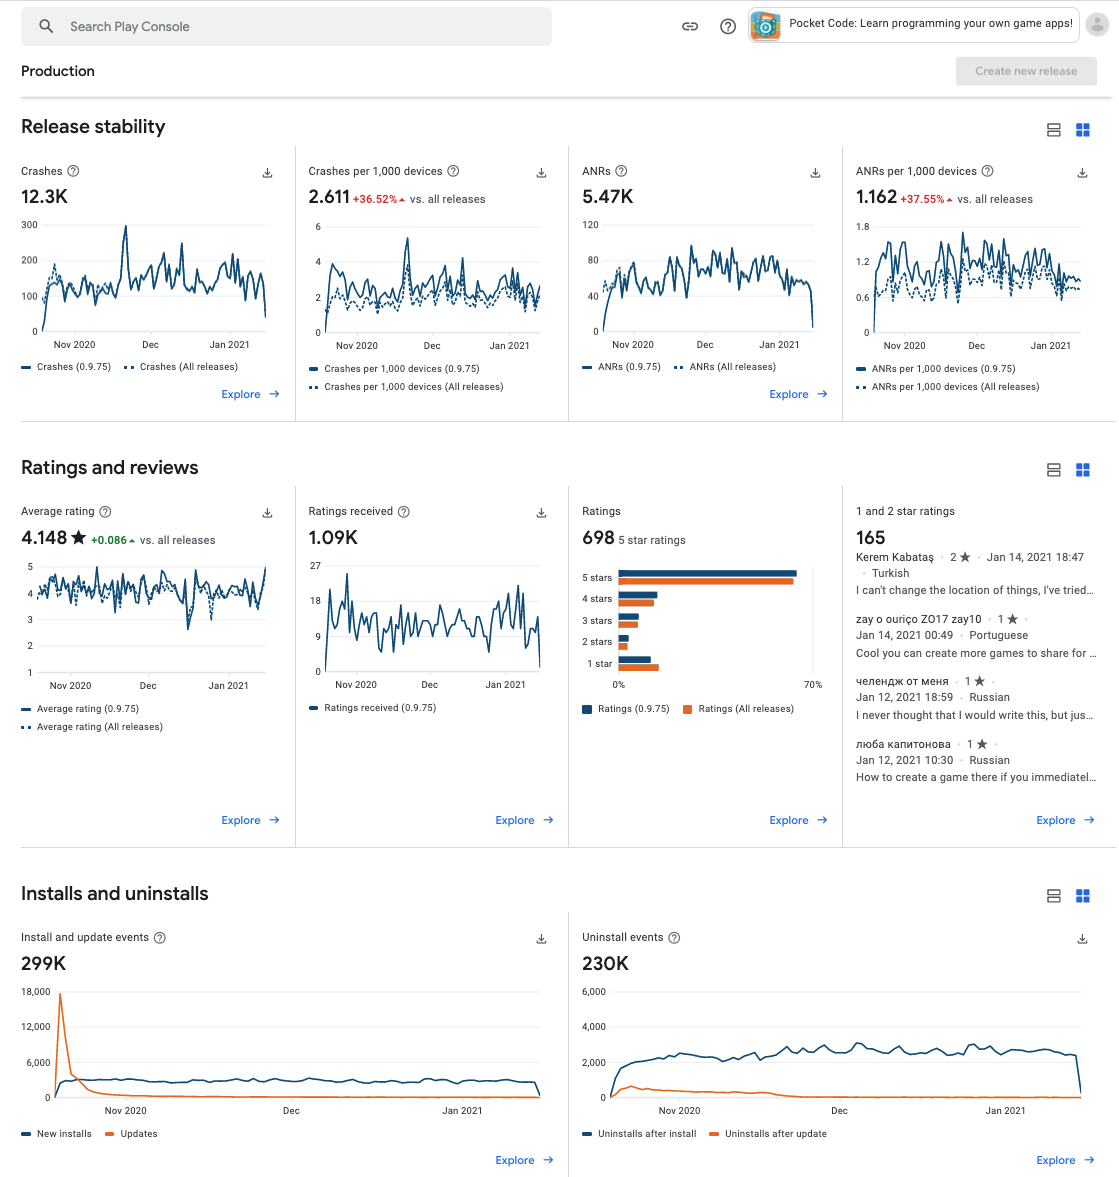
\includegraphics[width=12cm]{images/google-play-console/gpc-release-dashboard-pocketcode-v0.9.75-on2021-01-15.png}
    \caption{GPC: Release Dashboard for PocketCode V0.9.75}
    \label{fig:gpc-release-dashboard-pocketcode-v0.9.75}
\end{figure}

Figure~\ref{fig:gpc-release-dashboard-pocketcode-v0.9.75} provides an example of a recent release (0.9.75) of Pocket Code.


\subsubsection{Release Management: Release stability}


\subsubsection{Release Management: Ratings and Reviews}


\subsubsection{Release Management: Installs and uninstalls}




\subsection{Pre-launch reports}

~\url{https://stackoverflow.com/questions/48291106/security-warning-in-google-developer-console-pre-launch-reports-security-tab}

\subsection{Test channels}\label{subsection-test-channels}
MUST-DO complete this section.

\subsection{Android Vitals}
\subsubsection{Android Vitals UI}

\subsubsection{Peer Groups in Android Vitals}\label{android-vitals-peer-groups}
% Google calls them peer groups.
Android Vitals offers developers the option to define a peer group of between 8 and 12 other apps in the Google Play Store. The peer group can be edited up to 3 times per month according to the documentation, and changes seem to take immediate effect in terms of the reporting~\footnote{\url{https://support.google.com/googleplay/android-developer/answer/9324048}}.

The daily crash rate for the peer group can vary which is interesting in terms of observing variations in their overall crash-rate; Figure \ref{fig:pocketcode_peer_crash_rate_18_nov_2019} illustrates the daily change for one of the case studies: the Pocket Code Android app. It is not likely to be easy to determine which of those apps spiked (as the list can only be updated 3 times per month, editing the list and observing the difference has a low likelihood of unmasking the peer, the author will leave designing approaches for future research).

\begin{figure}[htbp!]
    \centering
    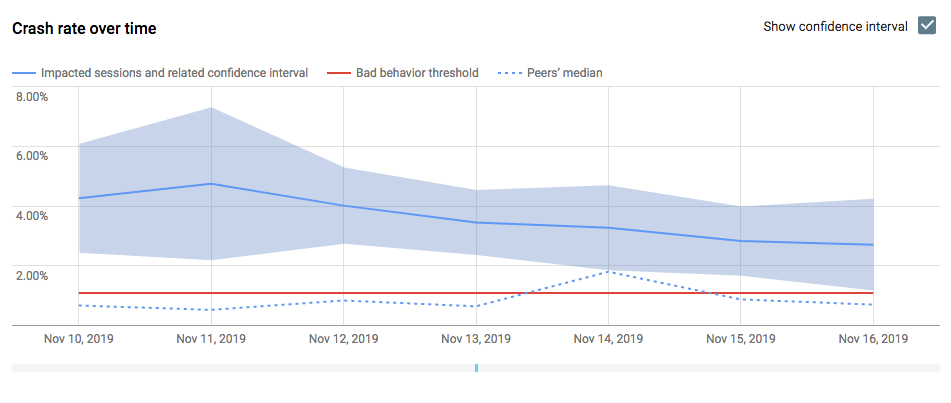
\includegraphics[width=\textwidth]{images/android-vitals-screenshots/peer-crash-rate-catrobat-18-nov-2019.jpg}
    \caption{Pocket Code peer crash-rate as of \nth{18} Nov 2019.}
    \label{fig:pocketcode_peer_crash_rate_18_nov_2019}
\end{figure}{}


\subsection{Monthly Report Files}

Google Play Console generates monthly reports, with the current month's report updated on a daily basis. 

%COULD_DO map screens or graphs to monthly report files.

\subsubsection{Access to the Monthly Report Files}
The reports are only made available for accounts which have 'global' read-only access\emph{`To access bulk reports, your "View app information" permission must be set to "Global."'}~\footnote{\url{https://support.google.com/googleplay/android-developer/answer/6135870\#export}}. Google explain why \emph{``Reports available on Google Cloud Storage use the same access restrictions that control data access on your Play Console. This means account users with access to areas of a Play Console account have access to the corresponding reports in Google Cloud Storage."}~\footnote{\url{https://support.google.com/googleplay/android-developer/answer/2528691}}  

\subsection{Google Play Console Revamp}
Google transitioned all users of Google Play Console from the previous version to a revamped version between June and 2nd November 2020. Developers were able to continue using the older version during the transition period by choosing the `classic' Play Console, this caused a URL parameter to be added~\texttt{\&noredirect} as demonstrated here
\url{https://play.google.com/apps/publish/?account=nnnnnnnnnnnnnn\&noredirect#AppListPlace} (the account number has been replaced to protect that account).

\section{Fabric Crashlytics}

\begin{itemize}
    \item History of Crashlytics:
    \item Crashlytics, one of several products incorporated into Fabric.
    \item Migration of Fabric from Twitter to Google.
    \item Firebase eclipses and supersedes Fabric
\end{itemize}

\url{https://status.firebase.google.com/incident/Crashlytics/20001}

Google retired the Fabric products, including Fabric Crashlytics on \nth{4} May 2020. They provided a range of similar product offerings in Firebase. For Fabric Crashlytics they continue to support the Fabric Client API (presumably so developers did not need to modify their apps to continue collecting crash data) however the reports differ in the Firebase Console, and developers had to explicitly migrate their apps from Fabric to Firebase. The Catrobat development team experienced insurmountable issues trying to migrate all bar one of their Android apps that used Fabric Crashlytics. Seemingly a common flaw also prevents the project team from adding Crashlytics to new apps in their Firebase Account. The workaround the team used was to create a second unrelated account in Firebase and to use that account to configure Crashlytics for apps. %SHOULD-DO discuss the final migration process with Wolfgang and the Android and iOS development teams.

\section{Firebase}
Firebase has come a long way from modest beginnings in 2011~\url{https://techcrunch.com/2012/04/19/firebase-post-launch/} and a change in focus~\url{https://techcrunch.com/2012/05/22/firebase-funding/} through acquisition by Google and further acquisitions~\url{https://www.crunchbase.com/organization/firebase}. Firebase analytics, incorporating Crashlytics, is now by far the most popular analytics library included in Android apps in Google Play. 

\subsection{Firebase Crashlytics}

\subsection{Firebase Analytics}

\section{Microsoft AppCenter}
App Center combines various tools and utilities and includes in-app mobile analytics and crash reporting. According to AppBrain is is installed in over 10 thousand apps and those apps have been downloaded over 23 billion times by \nth{25} November 2020.

\begin{table}[htbp!]
    \centering
    \footnotesize
    \begin{tabular}{rrr}
      Market share overall  &Market share in top apps &Market share in new apps  \\
      1.23\% of apps	  &7.20\% of apps &2.36\% of apps\\
      3.26\% of installs &8.10\% of installs &1.66\% of installs \\
    \end{tabular}
    \caption{AppBrain Statistics for Visual Studio App Center}
    \label{tab:appbrain_statistics_appcenter}
\end{table}

	

Statistics~\url{https://www.appbrain.com/stats/libraries/details/appcenter/visual-studio-app-center}

\textbf{Developer experience} The service and tools are freely available and there is a free pricing tier. The developer-oriented documentation is also freely available and includes~\href{https://docs.microsoft.com/en-us/appcenter/sdk/troubleshooting/android}{Android SDK troubleshooting}.

\textbf{Alerts and updates} 

\textbf{Account management} Access can be shared by the account holder.

\textbf{Integration of processes and practices} For development teams, no information is an island. Being able to annotate, track, integrate, and link information enables the tools and their reports to be integrated into software development practices such as bug reporting and tracking, cross-referencing of related work and activities and so so.

\emph{Dissecting a URL reference}
\url{https://appcenter.ms/users/ISNIT0/apps/Zipternet/crashes/errors/3418961070u}


\textbf{Data-pipeline-ability}


\textbf{Main features}
near real-time activity reporting.
email notifications of errors.

\href{https://docs.microsoft.com/en-us/appcenter/analytics/export}{\textbf{Export}}: App Center can continuously export raw Analytics data into Azure.


\section{Summary of Analytics Tools used in this research}
